\documentclass{article}

\usepackage{graphicx}
\usepackage{amsmath,amsfonts,amssymb}
\usepackage[colorlinks,bookmarks,bookmarksnumbered,allcolors=blue]{hyperref}
\usepackage[capitalise]{cleveref}
\usepackage[top=0.75in]{geometry}
\usepackage[dvipsnames]{xcolor}
\usepackage{amsmath} 
\usepackage{esvect}
\usepackage{hyperref}
\usepackage{graphicx}
\usepackage{subcaption}
\usepackage{stfloats}
\usepackage{array}
\usepackage{booktabs}
\usepackage{amsmath}

\begin{document}

\author{Joe Spencer}
\title{Rotor Analysis}
\date{October 12, 2022}
\maketitle

\subsubsection*{Methods}

A rotor's performance can be computed using  \hyperlink{BEM}{Blade Element Moment Theory}. This computation makes it possible to estimate how well a rotor will perform under various conditions without having to produce and test many prototypes. The Blade Element Momentum Theory calculations for this lab were conducted using BYU FLOW Lab's \href{https://flow.byu.edu/CCBlade.jl/stable/}{CCBlade.jl} header file. Used together with other julia header files, including \href{https://flow.byu.edu/Xfoil.jl/dev/}{Xfoil.jl}, A rotor's \hyperlink{CP}{Power}, \hyperlink{CT}{Thrust}, and \hyperlink{CQ}{Torque} distributions could be calculated, as well as its. \hyperlink{eta}{Efficiency}. \newline

Since it combines two theories to obtain the power, thrust, torque, and efficiency of an airfoil, CCBlade uses a system of equations to find them. The following equations are solved in this system to find the  \hyperlink{a}{Axial Induction Factor, $a$}, \hyperlink{a'}{Tangential Induction Factor}, and \hyperlink{phi}{Angle of Rotation, $\phi$}. A detailed description of other variables in this system of equations can be found in the \hyperlink{BEM}{Glossary}. \newline

\begin{equation}
\begin{aligned}
	\frac{1}{2} W^{2} N c C_{y} = 4 \pi U_{\infty} (1 - a) \times \Omega a' r^{2} \\
	\frac{1}{2} \rho W^{2} N c C_{x} = 4 \pi \rho [(a' \Omega r)^{2} + \Omega^{2}_{\infty} a (1 - a)] r \\
	\sin \phi = \frac{U_{\infty}}{W} (1 - a)
\end{aligned}
\end{equation}

Once these equations are solved, Axial Induction Factor and Tangential Induction Factor provide the ratios of increase and reduction in fluid flow velocity in the normal and tangential directions to the rotor. The angle of rotation provides the angle that the airfoil should form with the free stream velocity to achieve this result. The system of three equations shown is possible because it combines equations from both theories. \newline

After this system of equations is solved, the solutions for $a$, $a'$, and $\phi$ are used to find $C_{P}$, $C_{T}$, $C_{Q}$ and $\eta$ for an airfoil. The user can compare these values at different angles of attack to determine which advance ratio is best for an application. Different \hyperlink{T}{Twist Distributions}, \hyperlink{D/D}{Hub-to-tip Ratios}, \hyperlink{c}{Chord Distributions}, and \hyperlink{APC}{Propellor Types} can also be investigated to compare their performances. \newline

\subsubsection*{Results and Discussion}

This research led to a few discoveries that will be useful to optimize a rotor in the next assignment. These discoveries refined the size, shape, velocity, and blade quantity of rotors and gave insights into what results from changing each variable quantity. \newline

I first compared experimental rotor data with my own CCBlade computations. CCBlade.jl has a \href{https://github.com/byuflowlab/CCBlade.jl}{github Repository} containing some experimental data, which I used to test the functions I created. As shown in the Figure 1, 

\begin{figure}
  \centering
  \subfloat[Whatnot]{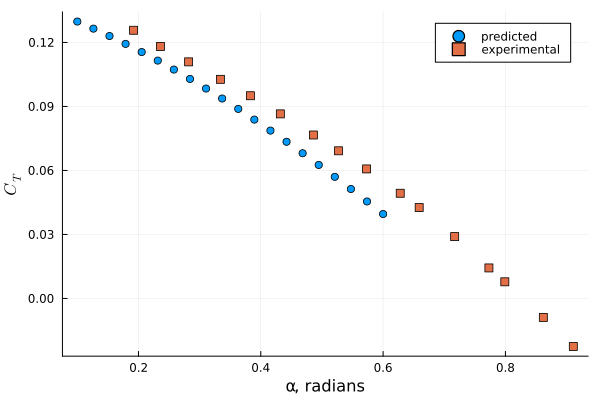
\includegraphics[width = .35\textwidth]{Plots/Figure_1.png}}
  \subfloat[Whatnot]{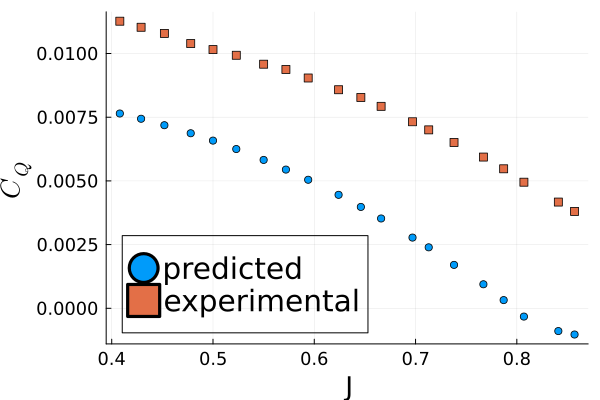
\includegraphics[width = .35\textwidth]{Plots/Figure_2.png}}

  \subfloat[Whatwhat]{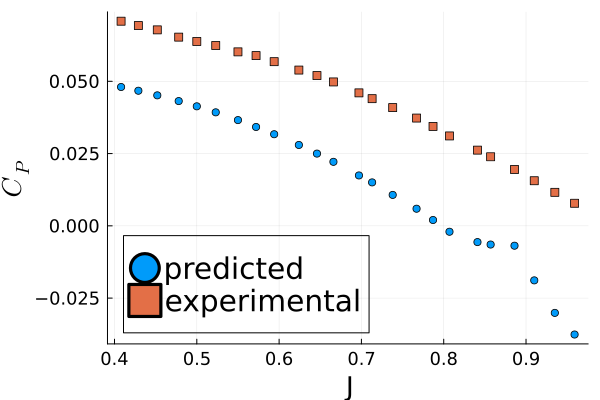
\includegraphics[width = .35\textwidth]{Plots/Figure_3.png}}\hspace{1em}
  \subfloat[Whatsit]{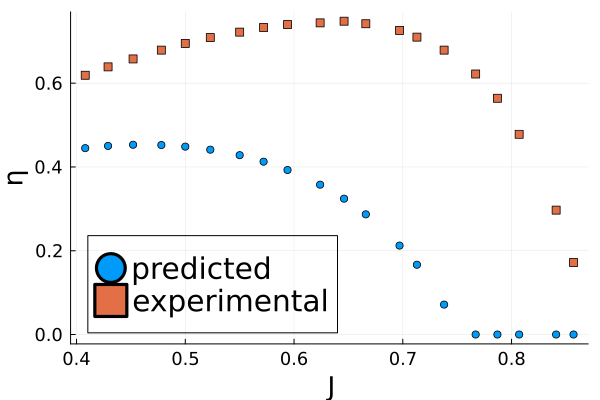
\includegraphics[width = .35\textwidth]{Plots/Figure_4.png}}
  \label{fig:1}
  \caption{Testing BEM Output Against Experimental Data. These plots show that although there are some differences, the Blade Element Momentum code provides a faithful estimate of the constants experienced by a rotor.}
\end{figure}

\href{https://github.com/JoeSpencer1/497R-Projects/blob/Airfoil-Analysis/Airfoil_Functions.jl}{header file}
The \hyperlink{BEM}{Blade Element Momentum Theory}

Axial induction factor $a$ Tangential induction factor $a'$

\clearpage

\section{Glossary}
\begin{itemize}
	
	\item \hypertarget{J}{Advance Ratio, $J$} - A rotor's Advance Ratio is a non-dimensional term. It describes the ratio how quickly a rotor is moving relative to the fluid flowing past it. A high advance ratio signifies that either the fluid is moving quickly or the rotor is moving slowly. It is described by the following equation, in which $V_{a}$ is the free stream fluid velocity, $n$ is the rotational velocity, and $D$ is the rotor diameter.
	\begin{equation}
	\begin{aligned}
		J = \frac{V_{a}}{n D}
	\end{aligned}
	\end{equation}
	
	\item \hypertarget{phi}{Angle of Rotation, $\phi$} - The Angle of Rotation, sometimes denoted by the Greek letter $\phi$, is the angle between the freest stream velocity and the velocity of the airfoil as it rotates. It is used in \hyperlink{BEM}{Blade Element Momentum Theory} calculations.

	\item \hypertarget{a}{Axial Induction Factor, $a$} - The Axial Induction Factor is the ratio of the reduction in air velocity at an airfoil to its free stream velocity.
	
	\item \hypertarget{BEM}{Blade Element Momentum Theory} - The theory used to calculate local forces on a propellor or wind turbine blade. It employs both \hyperlink{BET}{Blade Element Theory} and \hyperlink{MT}{Momentum Theory}. These equations are used to recursively find the \hyperlink{a}{Axial Induction Factor, $a$}, \hyperlink{a'}{Tangential Induction Factor}, and \hyperlink{phi}{Angle of Rotation, $\phi$}
	\begin{equation}
	\begin{aligned}
		\frac{1}{2} W^{2} N c C_{y} = 4 \pi U_{\infty} (1 - a) \times \Omega a' r^{2} \\
		\frac{1}{2} \rho W^{2} N c C_{x} = 4 \pi \rho [(a' \Omega r)^{2} + \Omega^{2}_{\infty} a (1 - a)] r \\
		\sin \phi = \frac{U_{\infty}}{W} (1 - a)
	\end{aligned}
	\end{equation}
In these equations, $a$, $a'$, and $\phi$ are the previously mentioned axial and tangential induction factors and angle of rotation. The airfoil's apparent speed is represented by the letter $W$, $N$ is the number of propellers, $\rho$ is the fluid density, $c$ is the chord length, $C_{x}$ and $C_{y}$ are obtained by the equation below, $U_{\infty}$ is the fluid free velocity, $\Omega$ is the blade's angular speed, and $r$ is the radius to the tip of the blade.
	\begin{equation}
	\begin{aligned}
		C_{x} = c_{l} \cos{\phi} + c_{d} \sin{\phi} \\
		C_{y} = c_{l} \sin{\phi} + c_{d} \cos{\phi}
	\end{aligned}
	\end{equation}
	
	\item \hypertarget{BET}{Blade Element Theory} - Blade Element Theory calculates the forces on a turbine blade by dividing it into finite pieces and summing the forces on all of these pieces. This theory determines the induced velocity and efficiency of a point along a blade using these equations:
	\begin{equation}
	\begin{aligned}
		v_{i} = \sqrt{\frac{T}{A} \frac{1}{2 \rho}} \\
        		\eta = \frac{\tan{\phi}}{\tan{(\phi + \gamma)}}
	\end{aligned}
	\end{equation}
In these equations, $v_{i}$ is the uniform induced velocity across the disk, $T$ the thrust it experiences, $A$ is its area, $\rho$ is the air density, $\phi$ is the angle to the airfoil's plane of rotation as it moves forward, and $\gamma$ is the difference between $\phi$ and $\beta$, what the airfoil's actual angle of rotation would be if it were stationary.

	\item \hypertarget{c}{Chord Distribution} - The Chord Length Distribution shows the length of a rotor's chord at different angular positions around itself. An airfoil with a constant angle of attack $\alpha$ as it generates lift has an elliptic chord distribution.
	
	\item \hypertarget{CP}{Coefficient of Power, $C_{P}$} - A propellor's Coefficient of Power signifies how efficient a wind turbine is. It is the ratio of the power generated by a wind turbine to the total power of the wind flowing through it. The power generated or absorbed by an airfoil can be described by the following equation, where $P$ is power, $C_{P}$ is the coefficient of power, $\rho$ is fluid density, $n$ is the velocity in revolutions per second, and $D$ is the propellor diameter. The Power Coefficient and the \hyperlink{CT}{Torque Coefficient} are proportional to each other by a factor of $2\pi$.
	\begin{equation}
	\begin{aligned}
		P = \rho n^{3} D^{5} C_{P} \\
		C_{P} = 2 \pi C_{Q}
	\end{aligned}
	\end{equation}
	
	\item \hypertarget{CT}{Coefficient of Thrust, $C_{T}$} - A rotor's Thrust Coefficient determines how much thrust in the forward direction an airfoil experiences. Thrust force is directly opposite drag. Please note the similarities and differences between the thrust equation and the \hyperlink{CP}{power equation}.
	\begin{equation}
	\begin{aligned}
		T = \rho n^{2} D^{4} C_{T}
	\end{aligned}
	\end{equation}
	
	\item \hypertarget{CQ}{Coefficient of Torque, $C_{Q}$} - A rotor's Torque Coefficient defines how much torque it will experience. A propellor's torque is given by the following equation, in which $Q$ represents torque, $\rho$ is the fluid density, $n$ is the velocity in revolutions per second, $D$ is the diameter, and $C_{Q}$ is the coefficient of torque. The Torque Coefficient and the \hyperlink{CP}{Power Coefficient} are proportional to each other by a factor of $2\pi$.
	\begin{equation}
	\begin{aligned}
		Q = \rho n^{2} D^{5} C_{Q} \\
		C_{Q} = \frac{C_{P}}{2 \pi}
	\end{aligned}
	\end{equation}
	
	\item \hypertarget{eta}{Efficiency, $\eta$} - The Efficiency of a rotor can be described by the following equation, in which $J$ is the rotor's \hyperlink{J}{Advance Ratio}, $C_{T}$ is its \hyperlink{CT}{thrust coefficient}, and $C_{P}$ its \hyperlink{CP}{power coefficient}:
	\begin{equation}
	\begin{aligned}
		\eta = J \frac{C_{T}}{C_{P}}
	\end{aligned}
	\end{equation}
	
	\item \hypertarget{D/D}{Hub-to-Tip Ratio} - A rotor's Hub-to-Tip Ratio divides the distance along the blade that is actually exposed wind by the entire length of the blade. This needs to be taken into account when calculating constants like the airfoil's \hyperlink{lambda}{tip speed ratio}.
	
	\item \hypertarget{MT}{Momentum Theory} - Momentum Theory defines the power required to produce sufficient thrust to maintain momentum in a blade by the following equation, where $T$ is thrust, $\rho$ is density, $A$ is disc area, and $P$ is power:
	\begin{equation}
	\begin{aligned}
        		P = \sqrt{\frac{T^{3}}{2 \rho A}}
	\end{aligned}
	\end{equation}
	
	\item \hypertarget{APC}{Propellor Identification} - A Propellor is identified by 2 numbers, which represent its diameter and its pitch, both in inches. For example, an APC 10 x 7 propellor is made by Advanced Precision Composites. It has a 10-inch diameter and a 7-inch pitch per revolution.
	
	\item \hypertarget{sigma}{Rotor Solidity, $\sigma$} - Rotor Solidity describes the ratio of a turbine's chord length, $c$, to its spacing, $s$. This is found by the following equation, in which $n_{b}$ is the number of blades, $r_{h}$ is the hub radius, and $r_{t}$ is the tip radius.
	\begin{equation}
	\begin{aligned}
		\sigma = \frac{c}{s} = \frac{c n_{b}}{2 \pi \sqrt{\frac{r^{2}_{h} + r^{2}_{t}}{2}}}
	\end{aligned}
	\end{equation}
	
	\item \hypertarget{a'}{Tangential Induction Factor, $a'$} - The Tangential Induction Factor is the ratio of the increase in air velocity tangential to the airfoil to its free stream velocity.
	
	\item \hypertarget{lambda}{Tip Speed Ratio, $\lambda$} - A wind turbine's Tip Speed Ratio is the inverse of its \hyperlink{J}{Advance Ratio, $J$}. It represents the ratio of the speed of the tip of a turbine blade, or $\omega R$, to the wind speed, $v$.
	\begin{equation}
	\begin{aligned}
		\lambda = \frac{\omega R}{v} = \frac{\pi}{J}
	\end{aligned}
	\end{equation}
	
	\item \hypertarget{T}{Twist Distribution} - Twist distribution along a wing redirects where air flows past it. This causes changes in both the magnitude and location lift and drag forces it experienced as air flows past it.
	
\end{itemize}

\end{document}